% Created 2010-04-22 Thu 14:10
\documentclass[11pt,a4paper,oneside,draft]{book}
\usepackage[utf8]{inputenc}
\usepackage[T1]{fontenc}
\usepackage[draft=false]{hyperref}
\usepackage[english,nynorsk]{babel} % or whatever language
\usepackage{apacite} % after babel
\usepackage{natbib}
\usepackage{graphics}
\usepackage{fixme}

\usepackage{amsmath} % for \operatorname

\usepackage{linguex} 

\usepackage{pslatex}
% \usepackage{pdfsync} % bug with glosses ( \exg. in linguex )

\usepackage{tikz-qtree}
\usepackage{avm}
\avmfont{\sc}
\avmoptions{sorted,active}
\avmvalfont{\rm}
\avmsortfont{\scriptsize\it}
\usepackage{algorithm2e}
\SetAlgorithmName{Funksjon}{fn}{liste over psevdokode}
%\SetAlgoFuncName{Funksjon}{} % for some reason gets no numbering TODO

\newcommand{\xbar}{$\rm\overline{X}$}
\newcommand{\F}[2]{\textsc{#1}\ensuremath{_{#2}}}
\newcommand{\OBLben}{\F{obl}{ben}}
\newcommand{\OBJben}{\F{obj}{ben}}
\newcommand{\OBJ}{\F{obj}{}}
\newcommand{\ADJ}{\F{adj}{}}
\newcommand{\XCOMP}{\F{xcomp}{}}
\newcommand{\SUBJ}{\F{subj}{}}
\newcommand{\PRED}{\F{pred}{}}
\newcommand{\falign}{\ensuremath{\operatorname{\emph{falign}}}}
\newcommand{\fpairs}{\ensuremath{\operatorname{\emph{fpairs}}}}

\title{Syntaktisk informert frasesamanstilling }
\author{Kevin Brubeck Unhammer}
\date{22/04, 2010}

\begin{document}

\maketitle

\setcounter{tocdepth}{4}
\tableofcontents
\vspace*{1cm}


\listoffixmes
\chapter{Introduksjon (+ samandrag/abstract)}
\label{sec-1}

Denne masteroppgåva utforskar kva det vil seie at to uttrykk er
omsetjingar av kvarandre, og korleis me automatisk kan generere og
evaluere samanstilling (\emph{alignment}, lenkjing) av uttrykk som står i
eit slikt omsetjingsforhold. Omsetjingsforhold finn me mellom
setningar i kontekst på ulike språk, men me kan au finne ulike typar
ekvivalensforhold (samanstillingar) mellom frasar innanfor setningane,
og mellom andre lingvistiske skildringar av setningane.

Det at me kan omsetje mellom slike skildringar (t.d. trekkstrukturane
til HPSG eller LFG) gjer det tydeleg at me arbeider med ein \emph{modell} av
språket; ulike skildringar kan vere sanne innanfor modellen, utan at
modellen er lik språket. Sjølve omsetjingsforholdet er au ein
teoretisk storleik, og ulike kriterium kan leggast til grunn for å
kalle to uttrykk omsetjingar av kvarandre. \citet{samuelsson2006pap}
nyttar t.d. reint semantiske kriterium, utan krav om syntaktisk
likskap, i deira manuelle samanstilling; medan samanstillinga planlagt
i XPar-prosjektet \citep{xpar2008rcn}, som kjem via
f-struktur-parallellismen\footnote{Eg~går~her~ut~frå~at~lesaren~er~kjend~med~grunnleggjande~LFG-terminologi.},
i større grad krev syntaktisk likskap.

Automatiske metodar for tekstsamanstilling kan nyttast til ulike
metodar for maskinell omsetjing, i tillegg til oppbygging av
parallelle korpora for meir teoretiske språkstudie. I samanheng med
XPar-prosjektet \citep{xpar2008rcn} har eg sett på metodar for
automatisk frasesamanstilling, dvs. for å finne omsetjingsforhold
mellom fleire ord. Dei første metodane for dette kom frå statistisk
maskinomsetjing, der ein berre nytta sannsyn av N-gram-omsetjingar,
utan nokon form for syntaktisk informasjon.  \citet{samuelsson2007apa}
skildrar ein metode kor frasesamanstilling blir oppnådd
vha. ordsamanstilling på ein parallell trebank der berre N-gram som
svarer til ein syntaktisk node blir samanstilt som
frasar. \citet{tinsley2007ept, hearne2008ccd} viser at slike
syntaktisk motiverte metodar kan forbetre frasebasert stokastisk
maskinomsetjing (\emph{PBSMT}). I XPar vil ein finne ut om
frasesamanstilling kan forbetrast ved å utnytte det at
LFG-grammatikkane for dei ulike språka er skrivne med same prinsipp
lagt til grunn; to parallellstilte setningar bør ha f-strukturar som
er like nok til at me kan samanstille frasar ved hjelp av likskapen
mellom f-strukturane. Sidan avbildinga frå c-strukturnodar til
f-struktur er mange-til-ein, kan me innanfor eitt tre ha fleire N-gram
per f-strukturhovud; slike relasjonar får me ikkje fram i metoden til
\citet{samuelsson2007apa}. Eg vil i masteroppgåva prøve å samanlikne
desse metodane, m.a. i forhold til dei ikkje-kontinuerlege
konstituentane til språk som georgisk, og utfordringane ved
samanstilling av språk med stor typologisk avstand.

\section{Framgangsmåte og ressursar}
\label{sec-1.1}

I \citet[s.~5--6]{xpar2008rcn} finn me følgjande hypotese:
\fxnote{siter heller den nye artikkelen}

\begin{quote}
On the basis of monolingual treebanks constructed from a parallel
corpus by means of parallel grammars it will be possible to achieve
automatic word and phrase alignment with significantly higher
precision and recall than hitherto achieved through other means.
\end{quote}

kor «parallel grammars» her krev parallellisme i båe f-struktur og
c-struktur. Eg vil konsentrere meg om å gjere ei samanlikning mellom,
på den eine sida, ein metode som nyttar enkel frasestrukturannotasjon
kombinert med ei ordsamanstilling for å finne frasesamanstillinga
(\emph{tremetoden}, basert på \citet{samuelsson2007apa}); og på den andre
sida ein metode som i tillegg nyttar f-struktur-informasjon frå desse
parallelle grammatikkane (\emph{LFG-metoden}).

Eg kjem til å nytte språka georgisk og norsk i samanlikninga,
hovudsakleg fordi dei er svært ulike syntaktisk og morfologisk.
Georgisk har t.d. mykje friare ordfølgje og rikare morfologi
(inkludert valensaukande mekanismar som \emph{applikativ}). 

Sidan eg ikkje har tilgang på ferdig setningssamanstilt georgisk-norsk
parallelltekst, blir det vanskeleg å køyre den statistiske
ordsamanstillinga som er vanleg som første steg i tremetoden (utan
ein god del forarbeid). Difor kjem eg til å konsentrere meg om eit
testkorpus
kor eg manuelt gjer ordsamanstillinga. Eg veit heller ikkje enno om
nokon statistisk parser av høg kvalitet for georgisk, men testkorpuset
vil vere ferdig parsa med LFG-parseren frå \citet{meurer2008cgg}, slik
at c-strukturane kan fungere som den syntaktiske annotasjonen i
tremetoden. Oppgåva blir altså å finne ut kva for bidrag informasjonen
på f-strukturnivået kan gi til samanstillinga, og kva for problem ein
støyter på.

Eg vil prøve å implementere testversjonar av LFG-metoden for
frasesamanstilling i eit passande programmeringsspråk.

\section{Frasesamanstilling frå f-struktur}
\label{sec-1.2}

Men om me har f-strukturane til to omsette setningar, burde det
kanskje vere mogleg å finne ei f-struktursamanstilling først og så
finne ordsamanstillinga ut frå denne. Tanken er at me frå to
f-strukturar som skildrar omsette setningar, kan
\begin{enumerate}
\item lage ei samanstilling mellom relevante deler av f-strukturane,
\item nytte denne funksjonelle samanstillinga til å finne ei
   frasesamanstilling, ved å følgje avbildinga frå f-struktur til
   c-struktur ($\phi{}^{-1}$).
\end{enumerate}
Eitt problem som byr seg er: kva for «deler av f-strukturane»? I det
minste må me kunne kople det opp mot c-strukturnodar; så \PRED-element
bør i det minste ha lenkjer, medan t.d. tempus og aspektuell
informasjon kanskje er mindre viktig. Men kva kan ignorerast? Vil det
oppstå tilfelle då me bør vekte visse element? (Dvs., må me nokon gong
disambiguere med slike andre element?)

Vidare må me vite \emph{korleis} me samanstiller desse delene. Me kan
t.d. byrje med å kople ytterste \PRED{} frå kvart språk, og så
rekursivt kople \PRED{} i dei relevante
substrukturane\footnote{Dette~krev~sjølvsagt~at~ytre~\PRED{}~faktisk~korresponderer~i~samanstilte~setningar,~ein~ikkje-triviell~påstand.}. Gitt
ein funksjon $i$ som returnerer indeksen til ein f-(sub)struktur, kan
eit førsteutkast til ei \emph{f-samanstilling}, samanstilling på
f-strukturnivå, sjå slik ut:

\[
\falign(f_{1}, f_{2}) =
\{ (i(f_{1}(\PRED)), i(f_{2}(\PRED))) \}
\cup
\bigcup_{g_{1},g_{2}\in \fpairs(f_{1},f_{2})} \falign(g_{1}, g_{2})
\]

\falign{} vil gi ei mengd av par av indeksar, kor kvart par altså er
samanstilt. Ein føresetnad her er at me i tillegg veit kva for par av
substrukturar som er «relevante» ($\fpairs(f_{1},f_{2})$).

Sjølv om f-strukturar abstraherer frå skilnadene i korleis ulike språk
nyttar ordgruppering og ordform til å kode syntaktiske forhold
\citep[s.~14]{bresnan2001lfs}, vil det likevel oppstå forskjellar i
f-strukturane til to parallellstilte setningar i eit korpus; båe
pga. «omsetjarfridom» og det at ulike språk nyttar ulike syntaktiske
funksjonar til å uttrykkje det same konseptet. I
f-struktursamanstillinga til \citet[s.~40]{riezler2006gmt} får dei
t.d. ei lenkje frå ein \XCOMP{} på tysk til eit \OBJ{} på
engelsk. Skal ein algoritme gå frå f-strukturar til frasesamanstilling
må han i det minste vere robust nok til å takle slik mangel på
samsvar. Til å byrje med kan me tenkje oss at \fpairs{} gir alle par
av GF-ar som har same plass i
argumentstrukturen\footnote{Ved~å~nytte~argumentplass~kan~me~enkelt~få~til~lenkjer~mellom~GF-ar~med~ulike~namn,~som~vist~i~dømet.}
til predikatet, så viss 'sein$\langle$\SUBJ,\XCOMP$\rangle$' står i
$f_{1}$ og 'have$\langle$\SUBJ,\OBJ$\rangle$' i $f_{2}$, vil \fpairs{}
i det minste returnere
$\{(f_{1}(\SUBJ),f_{2}(\SUBJ)),(f_{1}(\XCOMP),f_{2}(\OBJ)),...\}$.
Men om me ikkje har slikt samsvar i argumentstrukturar, vil \fpairs{}
ha ein vanskelegare jobb.

Eit større problem er nok adverbial (elementa i \F{adjunct}\{\}), kor
f-strukturane ikkje gir like greie hint om kva for substrukturar som
høyrer
saman\footnote{Det~er~mogleg~at~f-samanstillinga~av~adverbial~kan~tene~på~informasjon~frå~(og~difor~bør~skje~etter)~samanstillinga~av~frasane~som~projiserer~argumentfunksjonane.}. Ein
del av masteroppgåva vil altså vere å komme med forslag til funksjonen
\fpairs{}.


f-samanstillinga kan nyttast til å gi ein samanstilling av frasane dei
representerer. $\phi^{-1}$ gir no ei samanstilling mellom funksjonelle
domene i c-strukturane, me har t.d. ei lenkje mellom domenet
$d_{1}=\{X, Y, Z\}$ på språk 1 og $d_{2}=\{U, V, W\}$ på språk 2. Kvar
node frå $d_{1}$ vil kunne (symmetrisk) samanstillast med ein (eller
ingen) frå $d_{2}$.

Her kan me utnytte det at frasestrukturane i dei ulike grammatikkane
er tufta på same X-bar-prinsipp. Ein $XP\in d_{1}$ skal sannsynlegvis
samanstillast med ein $YP\in d_{2}$ (der $X$ og $Y$ gjerne er same
symbol, men au kan vere t.d. $V$ og $I$). I tillegg skal høge nodar
sannsynlegvis samanstillast med andre høge nodar, der alt anna er
likt, medan mangel på samsvar i samanstillinga til døtre kan føre til
at mornodar ikkje skal samanstillast; ein formalisering dette steget,
med diskusjon rundt problema, vil au inngå i masteroppgåva.

\chapter{Bakgrunn og relaterte metodar}
\label{sec-2}

\begin{itemize}
\item reine N-gram-samanstillingar, dependensbaserte
\item ulike formål for samanstilling gir ulike metodar
\item kort introduksjon til LFG
\end{itemize}
Frasesamanstilling er eit nytt felt. Det finst allereie veldig gode
system for automatisk setningssamanstilling, og automatisk
samanstilling av ord har komme langt, men nivåa mellom ord og setning
ser ut til å by på fleire problem. Dei ulike tilnærmingane som finst
er prega av formåla til utviklarane.

Innanfor korpuslingvistikken har \citet{piao2001mwu} nytta enkel
kollokasjonsinformasjon for å først finne sannsynlege nominale frasar
på engelsk og kinesisk, og så samanstille desse (ein metode kalla
«chunking»); her er evalueringsgrunnlaget rett og slett ein manuell
gjennomgang av dei mest sannsynlege omsetjingane dei får.

Men det er hovudsakleg innanfor stokastisk maskinomsetjing at ein har
forska på samanstilling av frasar. \citet{koehn2003spb} gir ein
grundig evaluering av ulike statistiske metodar for frasesamanstilling
til bruk i stokastisk maskinomsetjing. Dei nyttar
\textsc{Bleu}-systemet til å rangere resultata
\citep[Papineni~et~al.,~2001,~i][s.~51]{koehn2003spb}, som gir ei
rangering ved (N-grambasert) samanlikning med ferdig omsett tekst.

Den første metoden, \emph{AP}, er reint N-grambasert. Dei nyttar verktøyet
Giza++ \citep[Och~og~Ney,~2000,~i][s.~50]{koehn2003spb} til å indusere
ordsamanstilling frå eit setningssamanstilt korpus (vha. «modell 4»
for ordsamanstilling, utvikla ved IBM av \citet{brown1993msm}). Denne
samanstillinga er 1-til-n (t.d. eitt engelsk ord til to franske), så
dei finn ordsamanstilling for båe retningar og tek så snittet av alle
moglege N-gramsamanstillingar som ikkje er i konflikt med
ordsamanstillingane. Dei føyer så på ord frå unionen av desse
vha. nokre enkle heuristikkar.

Den andre metoden, \emph{Syn}, tek berre med dei frasane som står under
syntaktiske nodar i eit parsa korpus; frasesamanstillinga til \emph{Syn} er
ein delmengd av den i \emph{AP}. Denne syntaktisk informerte modellen gav ein
mykje dårlegare \textsc{Bleu}-skåre enn den reint N-grambaserte
modellen (faktisk dårlegare enn omsetjingane frå den originale modell
4, utan frasesamanstilling). Dei forklarer dette med den store mengda
uttrykk som ikkje utgjer syntaktiske konstituentar i følgje parseren
deira, men likevel konsekvent blir omsett til visse uttrykk på det
andre språket (t.d. «es gibt» på tysk til «there is» på engelsk).

Seinare resultat har vist at ein \emph{kombinasjon} av syntaktisk informerte
metodar med reint N-grambaserte modellar (dvs. i motsetning til å
berre fjerne samanstillingar mellom ikkje-konstituentar) kan auke
skåren i ein maskinomsetjingsevaluering, båe om ein som i \emph{Syn}-modellen
nyttar
frasestrukturinformasjon\footnote{\citet{samuelsson2007apa}~evaluerer~sitt~\emph{Syn}-liknande~system~ved~samanlikning~med~ein~manuelt~frasesamanstilt~gullstandard.},
men i endå større grad om ein nyttar dependendsinformasjon
\citep{hearne2008ccd}. F-strukturane til LFG gir ein slags
dependensinformasjon.

\citet{riezler2006gmt} utvikla ein metode for PBSMT med LFG-basert
generering på output-sida. Dei finn ei n-til-m-ordsamanstilling med
Giza++ som i metodane over, men parser i tillegg setningane i LFG. Dei
to moglege f-strukturane som liknar mest blir valt ut, og frå
ordsamanstillinga finn dei mange-til-mange-korrespondansar mellom
substrukturane i f-strukturane.

\chapter{Den ideelle frasesamanstillinga}
\label{sec-3}

\section{\textbf{SKRIV} LPT \textbf{:ROTETE:}}
\label{sec-3.1}

«a source word WS and a target word WT are taken to correspond
translationally only if (i) WT can in general (out of context) be
taken to be among the semantically plausible translations of WS, i.e.,
WT belongs to the set of `linguistically predictable translations
(LPT)' of WS, and (ii) WS and WT occupy corresponding positions within
corresponding argument structures.»

«a source phrase PHS and target phrase PHT are taken to correspond if
(i) they contain corresponding words, (ii) PHS contains no word or
phrase corresponding to a target word or phrase outside PHT, and
similarly (iii) PHT contains no word or phrase corresponding to a
source word or phrase outside PH.»

«It remains to be considered whether we should add the requirement
that PHS and PHT also occupy corresponding positions within
translationally corresponding argument structures, as we assume on the
level of word correspondences.»

«possibly also eliminate some of the initial links.» --
ie. non-monotonic phrase linking on top of the word linking.



\section{Introduksjon}
\label{sec-3.2}

I denne delen prøver eg å finne fram til kva som er den best moglege
frasesamanstillinga. Eg argumenterer for at «best» her må tolkast i
forhold til eit formål, og tek utgangspunkt i visse krav for
ordsamanstilling gitt i \citet{thunes2003eal}. Eg kjem fram til at når
formålet er utvikling av fasesamanstilte trebankar må ein revidere
kravet om likskap i argumentstruktur, og gir eit forslag til krav for
frasesamanstilling i trebankar.

\section{Kva er formålet med ei frasesamanstilling?}
\label{sec-3.3}

I frasebasert statistisk maskinomsetjing (PBSMT) skal ei
fraselenkje\footnote{Eg nyttar her termane \emph{lenkjing} og \emph{samanstilling} om
 kvarandre, i same tyding som det engelske \emph{alignment}; dette er
 ekvivalensforhold som me kan finne mellom lingvistiske
 \emph{representasjonar} (f-struktur, c-struktur) eller \emph{uttrykk} (ord,
 setningar). Lenkjing mellom dei siste altså er meir ateoretisk / datanært. } forbetre maskinomsetjing på eitt eller anna mål,
t.d. \textsc{Bleu}-skåren. \textsc{Bleu}-skåren samanliknar ferdig
omsett tekst (ein gullstandard) med det automatisk omsette, ved å
sjekke kor mykje N-gram-overlapp det er mellom tekstene. Ei
fraselenkje mellom N-grammet \emph{es gibt} og \emph{there is} (dvs. eit auka
sannsyn for å nytte slike par i omsetjinga) kan gi ein høgare endeleg
skåre i \textsc{Bleu}. Som vist i \citet{koehn2003spb} fekk dei ein
lågare \textsc{Bleu}-skåre når dei fjerna lenkjer mellom nodar som, i
følgje ein robust statistisk PCFG-parser, ikkje var syntaktiske frasar
(konstituentar). Dvs. at i figur \ref{fig:ikkjenode} vil lenkja vist
ved den prikkete lenkja bli fjerna frå mengda over moglege lenkjingar
om ein berre held seg til syntaktiske konstituentar, og
$p(es~gibt,~there~is)$ vil ikkje bli tilsvarande auka i den
statistiske omsetjingsmodellen. Sidan PBSMT, som skildra i
\citet{koehn2003spb}, er agnostisk til syntaktiske høve i
omsetjingssteget\footnote{Både omsetjingsmodellen og
språkmodellane er reint N-grambaserte her, og har difor ikkje nytte av
syntaktisk informasjon (i motsetning til syntaktisk informert
generering slik \citet{riezler2006gmt} implementerer). } er det for dei ingen grunn til å berre halde
seg til samanstilling mellom syntaktiske konstituentar; dei har i
utgangspunktet meir nytte av kollokasjonsinformasjon.

  \begin{figure}[htp]
    \vfill{} % how todo?
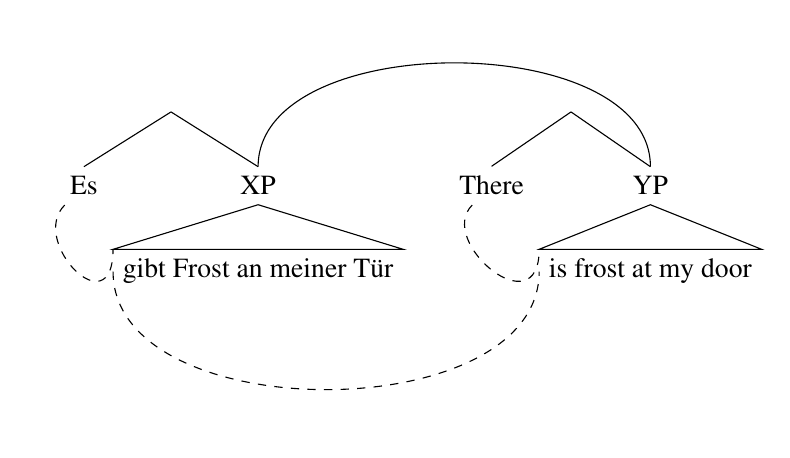
\begin{tikzpicture}
   \Tree [ [.\node(aDE){Es}; ]
    [.\node(pDE){XP};      
    \edge[roof]; \node(rDE){    gibt Frost an meiner Tür };  ] ] 
    \begin{scope}[shift={(2in,0in)}]
      \Tree [ [.\node(aEN){There};  ]
            [.\node(pEN){YP}; \edge[roof]; \node(rEN){ is frost at my door}; ] ]
          \end{scope}
          \draw[-] (pDE)..controls +(north:2) and +(north:2) .. (pEN); 
          \draw[dashed,-] (rDE.west)..controls +(south:2) and +(south:2) .. (rEN.west); 
          \draw[dashed,-] (aEN)..controls +(south west:1) and +(south:1) .. (rEN.north west); 
          \draw[dashed,-] (aDE)..controls +(south west:1) and +(south:1) .. (rDE.north west); 
\end{tikzpicture}
   \caption{N-gram-samanstilling versus syntaktiske frasar}
    \label{fig:ikkjenode}
  \end{figure}

Men sett no at me ikkje har som formål å nytte frasesamanstillinga til
reint N-grambasert omsetjing. Kva for \emph{lingvistiske} krav kan me stille
til å kalle to frasar samanstilte? I einkvar større parallelltekst vil
parallellstilte setningar ha visse syntaktiske og semantiske\footnote{Sidan eg føreset setningssamanstilte data, kjem eg ikkje inn på
 diskurs-/pragmatiske verknader, med mindre det kan vere mogleg
 å handsame desse innanfor setningen. }
omsetjingsskifte, t.d. leksikalisering av syntaktiske konstruksjonar
eller omvendt, endring av ordklasse, presisering/depresisering,
endringar i leksikale trekk (t.d. telleleg/utelleleg),
osb. \citep[s.~56--62]{munday2001its}, slik at den einaste
fullstendige, «perfekte» samanstillinga vil vere
identitetsfunksjonen. Me må godta ein del mangel på samsvar; kor mykje
me godtek blir då avgjort av formålet med samanstillinga.

Eg føreset her at eitt av formåla med samanstillinga er å kunne
oppdage korleis ulike språk realiserer semantiske roller syntaktisk;
då spesielt i forhold til hypotesane gitt i \citet[s.~7]{xpar2008rcn},
t.d. at «case marking might be useful to further determine a given
argument's semantic role». (Skal me finne det siste, må me altså kunne
samanstille frasar med ulik kasusmarkering, men ha krav om lik
tildeling av semantiske roller.)

Eit anna mogleg formål er å nytte desse frasesamanstillingane til
maskinomsetjing. \citet{riezler2006gmt} nyttar ein stokastisk
frasesamanstilling til å oppdage transfer-reglar for bruk i LFG-basert
generering i maskinomsetjing. Dette er reglar som omsett fragment av
ein f-struktur på kjeldespråket til f-strukturfragment på
målspråket. (Eit krav på utforminga av moglege transfer-reglar hindrar
at ein får reglar som lenkjar ikkje-konstituentar, eg kjem tilbake til
dette nedanfor.)  Samanstillinga utvikla her burde au kunne nyttast
til å finne slike transfer-reglar.

Nedanfor utviklar eg eit forslag til krav for ei frasesamanstilling,
med desse formåla i tankane. Om alle krava er moglege å implementere,
er eit separat problem.

\section{Krav / skrankar for frasesamanstilling i ein LFG-trebank}
\label{sec-3.4}


Samanstilte frasar bør ha nok semantisk likskap til å kunne opptre som
omsetjingar i liknande omgivnader
\citep[s.~74]{dyvik2009lmp}. \citet{thunes2003eal} gir nokre passande prinsipp
for å fastslå det som kan kallast \emph{omsetjingsmessig korrespondanse}, for
ordsamanstilling. Dette er prinsipp som skal gjelde for eit litt forskjellig
formål\footnote{\cite[s.~2]{thunes2003eal}: «Våre prinsipper er satt
opp for å tjene et bestemt formål, nemlig å samle inn data som metoden
i Semantic Mirrors skal anvendes på», ein metode for å automatisk
finne WordNet-liknande relasjonar frå parallelltekst. I denne metoden
vil det vere naturleg med høge krav til presisjon, men kanskje lågare
krav til dekning: speilmetoden skal finne leksikale semantiske forhold
som held på \emph{typenivå}, medan for trebanken er det viktigare korleis
me kan annotere eit \emph{token} av t.d. eit verb i ein viss VP i ei gitt
korpussetning. }, men som au «ligger nær opp til det vi intuitivt
mener er riktig» \citep[s.~2]{thunes2003eal}. Prinsippa blir nytta til
å lage ein gullstandard for ordsamanstilling (hovudsakleg for dei opne
klassene), og er definert ved å vise til kva for rolle eit argumentord
speler, eller kva for rolletildeling eit predikat eller modifiserande
ord gir. Så for å t.d. samanstille to verb må dei ha like mange
semantiske argument (men argumenta treng ikkje alle realiserast
syntaktisk) og dei må \emph{tildele same roller}; medan argumenta må \emph{spele same rolle}, og både argument og adjunkt må vere \emph{koreferente}. Lenkja
ord må vere del av frasar som speler same rolle i «det som er felles i
interpretasjonene av [dei to setningane]» \citep[s.~3]{thunes2003eal}.

Viss me tek utgangspunkt i det siste, vil det vere naturleg å i
tillegg lenkje desse frasane som speler same rolle i «det som er
felles i interpretasjonene».

Krava for ordsamanstillinga må au vere fylt for at desse frasane kan
samanstillast. Ein ordsamanstilling er altså naudsynt for ein
frasesamanstilling, og omvendt. Dette er berre motsetningsfylt om me
føreset at det eine er derivert av det andre; men dette har me ingen a
priori grunn til å gjere. Krava eg her utviklar bør i staden sjåast på
som \emph{skrankar} på moglege samanstillingar, på same måte som dei
modellteoretiske tolkingane av LFG og HPSG.

\citet{pullum2001dbm} gir ein god gjennomgang av forskjellen
mellom derivasjonelle (enumerative) grammatikkar og skrankebaserte
modellteoretiske grammatikkar, kor førstnemnde definerer \emph{mengder av uttrykk} ved avleiing frå startsymbol, medan sistnemnde gir skildringar
av \emph{enkeltuttrykk}. Ein modellteoretisk grammatikk kan i tillegg skildre
strukturen (eller dei moglege strukturane) til \emph{fragment} av setningar,
og denne strukturen er lik det bidraget som fragmentet tilfører
skildringa av heile setninga. Det tilsvarande er ikkje mogleg å gjere
derivasjonelt. \citet[s.~32--33]{pullum2001dbm} gir t.d. eit fragment
som kjem midt i eit høgreforgreina tre; ein derivasjonell skildring
ville måtte skildre treet over eller under, men utan informasjon om
kva som kjem til høgre eller venstre kan me ikkje (på ein
ikkje-vilkårleg måte) skildre subtreet utanfor fragmentet heilt fram
til terminal- eller startsymbol. 

Sidan ei frasesamanstilling er ei skildring av forhold mellom
setningsfragment vil det vere naturleg å skildre dei ønskelege
forholda som skrankar på moglege samanstillingar. Dette let oss au
setje skrankar på både frase- og ordsamanstilling sameleis, utan å
måtte ha krav om at den eine samanstillinga er fullstendig avleiia av
den andre; noko me ikkje har eit \emph{a priori} grunnlag for å seie. 

Sidan metoden er mynta på bruk i ein LFG-parsa trebank, og delvis vil
nytte denne parsen som datagrunnlag, er det naturleg å nytte same
konsept som blir nytta i LFG\footnote{I tillegg finst andre positive biverknader av ein LFG-basert
 frasesamanstilling for bruk i denne samanhengen, som at ein kan
 oppdage kor parallelle dei parallelle grammatikkane i
 ParGram-prosjektet \citep{butt2002pgp} faktisk er, på ulike nivå
 (leksikon og argumentstruktur, c-struktur, f-struktur). } (f-struktur, c-struktur,
endosentrisitetsprinsipp, \xbar{}-tre, osb.)  au i desse krava til den
«beste» frasesamanstillinga; i den grad LFG gir ein generaliserbar
skildring av syntaks, bør desse krava vere generaliserbare til andre
teoriar.

Eg byggjar vidare på krava frå \citet{thunes2003eal} nedanfor, men
kjem som nemnd med visse endringsforslag.

\section{Kva kan samanstillast?}
\label{sec-3.5}


Viss to uttrykk er samanstilt på setningsnivå (slik at me dimed kan gå
ut frå at dei er omsetjingar av kvarandre), og båe har ein
LFG-analyse, så har me iallfall tre ulike nivå kor me kan finne
ekvivalensforhold under setningsnivå:
\begin{enumerate}
\item mellom ord i setningane,
\item mellom f-strukturar,
\item mellom c-strukturnodar.
\end{enumerate}
Alle ord i setninga er \emph{kandidatar} for samanstilling med ord i
omsetjinga, men \emph{a priori} kan me ikkje utelukke at eit ord ikkje har ei
lenkjing, og me kan heller ikkje utelate mange-til-mange-lenkjing. Det
same gjeld nodane i c-strukturen.

\fxnote{i tillegg vil samanstilling av andre trekk vere endå eit steg
lenger vekk frå observerte data}

Når det gjeld f-strukturane er det ganske mange element me teoretisk
sett kunne ha samanstilt, t.d. enkelttrekk som bestemtheit eller dei
uordna mengdene med adjunkt, men det som er mest \emph{nyttig} er nok å
berre gjere samanstillingar der det er ei nær kopling til orda i
setninga. Sidan alle PRED-element i ein f-struktur unikt står for
predikerande ord, kan me -- gitt to samanstilte setningar -- la
\emph{kandidatane for samanstilling på f-strukturnivå} inkludere\footnote{I del \ref{SEC:fnord} kjem eg tilbake til spørsmålet om me vil
        inkludere visse f-strukturar utan PRED-element i kandidatane
        for samanstilling. }
alle desse PRED-elementa i f-strukturane til setningane. PRED-element
representerer semantiske bidrag som oftare er naudsyne på båe språk i
omsetjingar, medan andre f-strukturtrekk gjerne er valfrie på det eine
av språka; det er ikkje alle språk som har t.d. obligatorisk
kasusmarkering, og ein vil kanskje nytte trebanken til å oppdage
nettopp slik variasjon.  PRED-elementa er i tillegg gjerne enklare å
knyte direkte opp mot konkrete tekststrengen, medan t.d. aspekt
kanskje er umogleg å skilje frå tempus i affikset.

Eg føreslår følgjande føringar:

\ex. \label{f-links} Ei samanstilling av to PRED-element i f-strukturane tilseier at:
\a. \label{f-links-substr} f-strukturane til desse er lenkja,
\b. \label{f-links-words} orda i setningane som projiserer
   PRED-elementa tek del i ei samanstilling med kvarandre (kor andre
   ord kan vere involvert), og at
\c. \label{f-links-domain} iallfall dei øvste nodane i det funksjonelle
   domenet\footnote{Det funksjonelle domenet til ein f-struktur er gitt ved
 $\phi^{-1}$, inversen av c-til-f-strukturavbildinga, og tilsvarer dei
 nodane i c-strukturen som projiserer denne f-strukturen, t.d. ein
 VP-node med dominerande IP og CP
 \citep[s.~126]{bresnan2001lfs}. Sidan dette er inversen av ein
 funksjon, kan me ha diskontinuerlege konstituentar i same
 funksjonelle domene (fleire funksjonsargument som gir same verdi). } til f-strukturen er samanstilt.

(Underordna nodar i det funksjonelle domenet kan berre lenkjast om
visse krav, gitt nedanfor, er oppfylt. Me kan altså gjerne ha
c-strukturnodar som ikkje er lenkja til andre nodar.)

\fxnote{backe det med eksemplar i trebank; kople til adj-arg-lenkje}

Påstandane over må forsvarast. Punkt \ref{f-links-substr} og
\ref{f-links-domain} over seier at viss PRED-elementa projisert av
t.d. to verb i verbfrasar er lenkja, vil \emph{heile} VP-ane vere lenkja
(både VP-nodane som dominerer dei lenkja funksjonelle domena og
f-strukturane frå ytre PRED til verba), det er dette som gjer det til
ei fraselenkje; medan i følgje punkt \ref{f-links-words} vil denne
fraselenkja leie til at sjølve verba au er lenkja, ein sterkare
påstand sidan dette tilseier at \emph{PRED-samanstilling impliserer ordsamanstilling}. I visse tilfelle er dette heilt uproblematisk,
t.d. viss \emph{I slept down by the river} skal lenkjast med \emph{Eg sov nede med elva} vil me uansett lenkje \emph{slept} og \emph{sov}; dette kan gjelde
transitive verb au:

\ex. \a. The locusts have no king, just noise and hard language\\
     $\leftrightarrow$
     \b. Grashoppene har ingen konge, berre støy og krasse ord

\fxnote{der ADJUNKT ikkje er realisert, lenkjer me ikkje PRED.  skal
me då ikkje lenkje ord heller?}

\fxnote{PRED->ord :: iallfall\\
PRED<-ord :: ?\\
PRED<->ord\\
PRED, ord}

\emph{have/har} tek del i VP-samanstillinga \emph{have no king.../har ingen konge...}.

Som nemnd over; ordsamanstillinga treng ikkje vere ein-til-ein, det
punkt \ref{f-links-words} seier er at desse orda iallfall er ein del
av ein samanstilling med kvarandre (i \Last altså
VP-samanstillinga). Kanskje er dette ei mange-til-mange-lenkjing som
ikkje \emph{kan} reduserast til ein-til-ein-lenkjingar; eller kanskje er
det som i \Last mogleg å skilje ut delsamanstillingar, som
\emph{have/har}. Eg kjem tilbake til dette i del \ref{SEC:lik-argstr} om
argumentstruktur og adjunkt. 

\fxnote{avsnittet over er litt rotete TODO}

Alle nodar i c-strukturen (alle syntaktiske \emph{frasar/konstituentar} i
setninga) som kan koplast til PRED-haldande f-strukturar, vil altså
vere kandidatar for samanstilling på c-strukturnivå (dette inkluderer
diskontinuerlege konstituentar), men ikkje alle vil bli samanstilt.
\subsection{\textbf{TOGROK} finst det tilfelle der ordlenkjer ikkje impliserer PRED-lenkjer?}
\label{sec-3.5.1}

   hypotese: det er alltid slik at \\
   ordlenkjing av predikerande ord => PRED-lenkje
\section{\textbf{TOGROK} kva med ekspletivar? ingen PRED men heller ikkje C/F/I \textbf{:ROTETE:}}
\label{sec-3.6}

Kandidatane på f-strukturnivå må jo inkludere desse au\ldots{}
\section{\textbf{TODO} Gi enkelt døme kor alt fungerer \textbf{:ROTETE:}}
\label{sec-3.7}


\section{Funksjonsord}
\label{sec-3.8}

\label{SEC:fnord}
I tillegg kan me ha ord i setninga som ikkje tilsvarer PRED-element i
f-strukturen, typisk funksjonsord (t.d. \emph{som}, \emph{at}). Ved
endosentrisitetsprinsippa til \citet{bresnan2001lfs} er komplementet
til funksjonelle kategoriar (C, I, P) ein funksjonell ko-kjerne. 

\ex. \label{fnordkrav} Skal nodar for ord som ikkje projiserer
     PRED-element\footnote{Skal ein lenkje ordet \emph{som} (utan PRED) med ordet \emph{which} (med
 PRED)? Viss båe står under C i treet, kan det kanskje vere
 informativt med ein type «defekt» lenkje, sjølv om berre det eine
 ordet blir rekna for å vere eit innhaldsord. Frasane til deira
 funksjonelle domene vil uansett vere samanstilt via toppnodane
 (t.d. CP). } samanstillast, må følgjande krav vere oppfylt:
\a. det funksjonelle domenet (gitt ved komplementet) må vere
   samanstilt, og
\b. dei er båe c-strukturhovud.


Om \Last[a og -b] er oppfylt, kan me få samanstillinga vist i figur
\ref{fig:fnord}, og i dette tilfellet er \Last[b] oppfylt og \Last[a]
vil vere oppfylt om me kan samanstille \emph{cvimda} med \emph{det regnet}.

  \begin{figure}[htp]
   \vfill{} % how todo?
  
  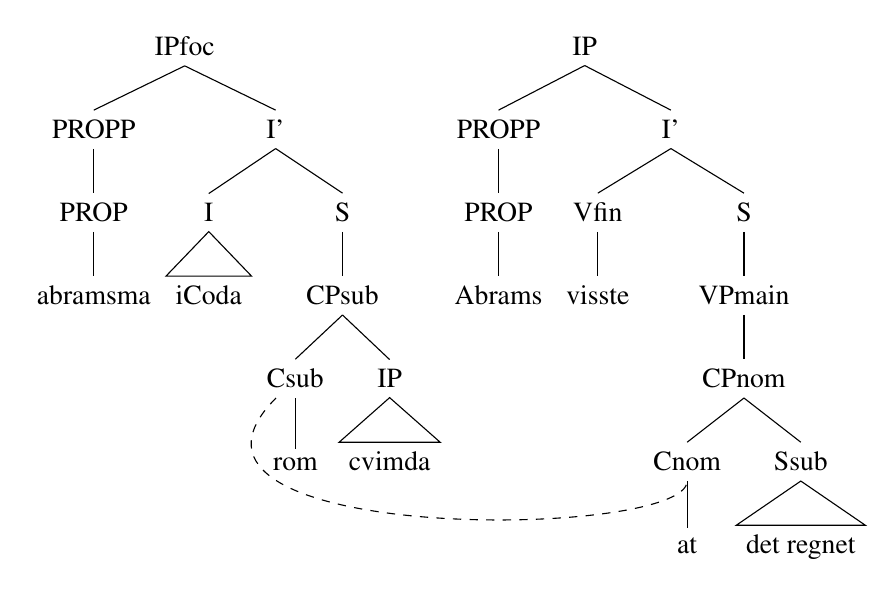
\begin{tikzpicture}
  \Tree
  [.IPfoc
    [.PROPP [.PROP abramsma ] ] 
    [.I' [.I \edge[roof]; {iCoda} ]
             [.S [.CPsub
                  [.\node(Csub){Csub};  rom ]
                  [.IP \edge[roof]; {cvimda} ]]]]]
      \begin{scope}[shift={(2in,0in)}]
  \Tree
  [.IP
    [.PROPP [.PROP Abrams ] ]
     [.I' [.Vfin visste ]
              [.S [.VPmain [.CPnom
                           [.\node(Cnom){Cnom};  at ] 
                            [.Ssub \edge[roof]; {det regnet} ]]]]] ]
  \end{scope}                      
  \draw[dashed,-] (Csub)..controls +(south west:3) and +(south:1) .. (Cnom) ;
  \end{tikzpicture}
  \caption{Mogleg samanstilling av funksjonsord mellom georgisk og norsk (bokmål)}
   \label{fig:fnord}
  \end{figure}
\subsection{\textbf{TOGROK} cvimda<PRO> men regne<>expletive -- lenkje? \textbf{:ROTETE:}}
\label{sec-3.8.1}


\section{Lenkjing av underordna c-strukturnodar}
\label{sec-3.9}

\label{SEC:subnode}

Toppnodane i eit lenkja funksjonelt domene i c-struktur (XP på språk
1, ZP på språk 2) vil ha ein informasjonsmessig korrespondanse, og kan
samanstillast. Men det er mogleg å samanstille to toppnodar i
funksjonelle domene i c-strukturen utan at nodane under (X', Z') er
samanstilt. Ein grunn til å ikkje samanstille desse underordna nodane,
vil vere viss spesifikator til X ikkje speler same rolle i tolkinga
som spesifikator til Z, dvs. viss YP og WP i figur \ref{fig:subnode}
ikkje er lenkja.


Me kan utelukke lenkjing av ikkje-konstituentar som \emph{there is} ved å
krevje at ei fullstendig samanstilling mellom to frasar må vere slik
at heile substrukturen au er samanstilt. \emph{There is} og \emph{Es gibt} i
figur \ref{fig:ikkjenode} kan då ikkje samanstillast åleine, men berre
som del av ei ytre frasesamanstilling.
Så når \emph{kan} me samanstille nodane som står under øvste node i
f-domenet?

\begin{figure}[htp]
   \vfill{} % how todo?
   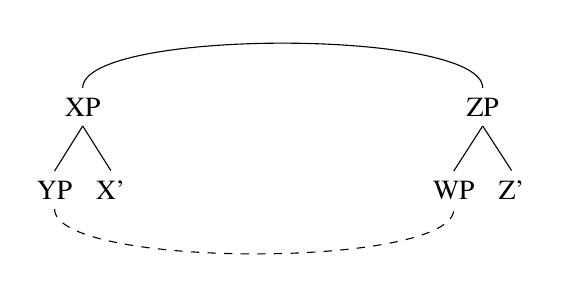
\begin{tikzpicture}
  \Tree  [.\node(XP){XP};  \node(YP){YP};  
                                    \node(X'){X'};   ]
      \begin{scope}[shift={(2in,0in)}]
  \Tree  [.\node(ZP){ZP};  \node(WP){WP};  
                                    \node(Z'){Z'};   ]
\end{scope}
\draw[-] (XP)..controls +(north:1) and +(north:1) .. (ZP) ;
  \draw[dashed,-] (YP)..controls +(south:1) and +(south:1) .. (WP) ;

\end{tikzpicture}
   \caption{Lenkjing av underordna c-strukturnodar}
   \label{fig:subnode}
  \end{figure}

I figur \ref{fig:subnode} der XP og ZP er lenkja, vil YP og WP -- i
kraft av å vere toppnodar i sine domene -- måtte ha ei lenkje i
f-strukturen for at c-strukturnodane kan lenkjast (det kunne jo
t.d. hende at f-strukturen projisert av YP samsvarte med den projisert
av Z', eller ein struktur under Z').

Om me skal lenkje Z' og X' i figuren over må dei respektive
spesifikatornodane vere lenkja. Me får då følgjande krav:

\ex. \label{subnodekrav} Krav for lenkjing av underordna
c-strukturnodar:
\a. c-strukturnodar som ligg under øvste node i to funksjonelle
    domena kan berre samanstillast med nodar som ligg innanfor desse
    domena,
\b. c-strukturnodar kan berre samanstillast om deira funksjonelle
    domene er lenkja på f-strukturnivå,
\c. om ein c-strukturnode X' som ikkje er toppnode i det funksjonelle
    domenet har ein søsternode YP, må YP vere samanstilt med ein
    søsternode til Z' for å samanstille X' og Z'


\Last[a] seier at om XP og ZP er samanstilt, der XP er t.d. OBJ til
IP, kan ikkje Z' samanstillast med SUBJ til IP osb., men berre til
nodar innanfor OBJ-domenet. \Last[c] påført figur \ref{fig:subnode}
seier altså at spesifikatornodane må vere lenkja for at X' og Z' skal
lenkjast (manglande søsternode på den eine sida vil au hindre
samanstilling).

I figur \ref{fig:fnord} er alle nodane under S vist i dei to trea i
same funksjonelle domene (kvar node under S er annotert med $\uparrow
= \downarrow$), så om dei funksjonelle domena er samanstilt (som krev
at \emph{rom cvimda} og \emph{at det regner} er samanstilt), vil \Last[a og -b]
vere oppfylt kva gjeld CP-komplementa -- lenkjinga går ikkje ut over
dei funksjonelle domena. Sidan Csub og Cnom er funksjonelle kategoriar
er dei au samanstilt via samanstillinga av S-nodane og føringane i
\ref{fnordkrav}, og \Last[c] er då oppfylt. \Last står altså ikkje i
vegen for å samanstille IP-en over \emph{cvimda} og Ssub.

I figur \ref{fig:ikkjesub} derimot \citep{mrs-suite}, kan me ikkje
samanstille I'-nodane. PRONP-noden, spesifikator på den norske sida,
er ikkje lenkja med nokon spesifikator på den georgiske sida. Den
informasjonen (her reint syntaktisk) som ordet \emph{det} tilfører IP, ligg
under I' på georgisk. Om me skulle lenkja I', måtte me altså hatt ein
georgisk spesifikator som var lenkja til den norske PRONP.

\begin{figure}[htp]
 \vfill{} % how todo?
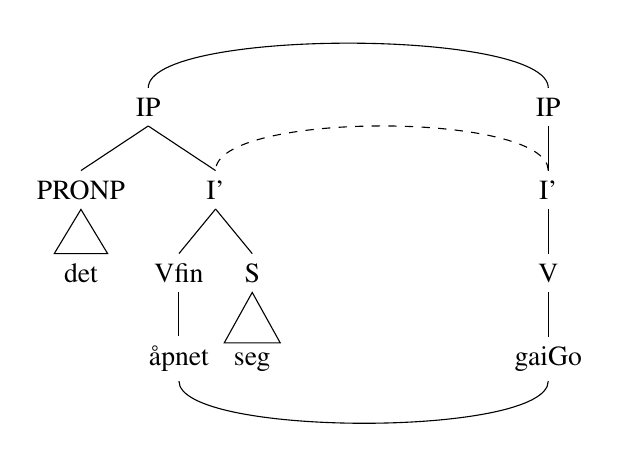
\begin{tikzpicture}
\Tree [.\node(IPb){IP}; 
  [.PRONP \edge[roof]; {det} ] 
  [.\node(Ibarb){I'};  [.Vfin \node(åpnet){åpnet};  ]
       [.S \edge[roof]; {seg} ] ] ]
      \begin{scope}[shift={(2in,0in)}]
\Tree [.\node(IPk){IP}; 
  [.\node(Ibark){I'};  [.V    \node(gaiGo){gaiGo};  ]
  ] ]
\end{scope}
 \draw[-] (IPk)..controls +(north:1) and +(north:1) .. (IPb) ;
  \draw[dashed,-] (Ibark)..controls +(north:1) and +(north:1) .. (Ibarb) ;
 \draw[-] (gaiGo)..controls +(south:1) and +(south:1) .. (åpnet) ;

\end{tikzpicture}
\caption{Umogleg samanstilling av funksjonsord mellom bokmål og georgisk}
 \label{fig:ikkjesub}
\end{figure}

\subsection{\textbf{SKRIV} døme! \textbf{:ROTETE:}}
\label{sec-3.9.1}

\subsection{\textbf{TOGROK} me$_{\mathrm{OBJ}}$ gusta X$_{\mathrm{SUBJ}}$ // I$_{\mathrm{SUBJ}}$ like X$_{\mathrm{OBJ}}$ ?? \textbf{:ROTETE:}}
\label{sec-3.9.2}

\subsection{\textbf{TOGROK} korleis finn me \emph{there is}-lenkjer då? \textbf{:ROTETE:}}
\label{sec-3.9.3}

(og kva skal me med dei?)

«Til gjengjeld vil me få lenkjer sjølv om me har mellomståande ord
(\emph{There} never \emph{is}) som opptrer utanfor N-grammet på det andre
språket.»

\section{\textbf{TOGROK} mange-til-mange-lenkjing i f-strukturane? \textbf{:ROTETE:}}
\label{sec-3.10}

    Eg er litt usikker på om me skal ha slike
    mange-til-mange-korrespondansar i f-strukturane; eg har rekna med
    at ei f-strukturlenkje \emph{impliserer} ei slags lenkjing mellom det som
    er innanfor f-strukturane; men i \citet{riezler2006gmt} er det i
    staden berre eit krav om at desse f-strukturane er lenkja i same
    transfer-regel.


\citet[s.~40--41]{riezler2006gmt} tillet mange-til-mange-lenkjing
mellom f-strukturar, så lenge alle f-strukturane som blir lenkja til
slutt opptrer i same transfer-regel. Frå følgjande setningspar:

\ex. Dafür bin ich zutiefst dankbar \\
     I have a deep appreciation for that

lenkjar dei \{\emph{zutiefst}\} med \{ \emph{a, deep, appreciation} \}, men
sidan \{\emph{appreciation}\} er samanstilt med \{\emph{dankbar}\}, må
transfer-regelen inkludere \{ \emph{zutiefst, dankbar} \} på den eine sida
og \{ \emph{a, deep, appreciation} \} på den andre.


\subsection{\textbf{SKRIV} Kva inneber ei mange-til-mange-lenkjing? \textbf{:ROTETE:}}
\label{sec-3.10.1}


\section{\textbf{SKRIV} Mangel på samsvar i syntaks og semantikk \textbf{:ROTETE:}}
\label{sec-3.11}

\cite[s.~5]{kruijffkorbayova2006agc} gir følgjande døme: 
\ex.  nikdy nebyl \\
      never was.not\\
      `has never been'

\emph{nebyl} blir «svakt» samanstilt med \emph{never}, men «sterkt» samanstilt med
\emph{has ... been} i deira system. I tillegg er det ein sterk samanstilling
mellom \emph{never} og \emph{nikby}.


\section{\textbf{TOGROK} Diskontinuerlege einingar \textbf{:ROTETE:}}
\label{sec-3.12}

\begin{itemize}
\item diskontinuerlege einingar \cite[s.~4]{cheung2002scg}
     \href{http://scholar.google.no/scholar.bib%3Fhl%3Dno&lr%3D&ie%3DUTF-8&q%3Dinfo:Qh_MRSftNZgJ:scholar.google.com/&output%3Dcitation&oe%3DMACINTOSH&oi%3Dcitation}{@books.google} -- skal dei eigentleg samanstillast? Kva for problem
     gir dei i forhold til c-strukturnivåsamanstilling?
\end{itemize}
\subsection{\textbf{TODO} døme på diskontinuerlege konstituentar som er lenkja \textbf{:ROTETE:}}
\label{sec-3.12.1}

\section{\textbf{TOGROK} Er «compounds» frasar? \textbf{:ROTETE:}}
\label{sec-3.13}

 \citep[p.~1]{giegerich2006aea}


\section{Lik ordklasse?}
\label{sec-3.14}

Ulike språk leksikaliserer same konsept på ulike
måtar. \citet[s.~3]{cheung2002scg} skriv at det engelske ordet
\emph{fulfilment} meir naturleg blir omsett til eit verb på kinesisk. Det
same gjeld t.d. \emph{solitude} omsett til norsk. Eit georgisk
verbalsubstantiv (\emph{masdar}) kan bli omsett til eit verb i infinitiv på
norsk\footnote{Det georgiske verbalsubstantivet (\emph{masdar}) er i følgje
        \citet[kap.~2.5]{aronson1990grg} ein \emph{nominal} form, det kan i
        motsetning til norske verbalsubstantiv og engelske gerundium
        ikkje ta objekt, men kan ha modifiserande substantiv i
        genitiv. }. Slike skifte mellom ordklassar er svært vanlege i
omsetjing\footnote{\citet[Catford~(1965),~i][s.~61]{munday2001its} gir ein gjennomgang av
slike \emph{klasseskifte}, og andre typar omsetjingsskifte. }.

Me kan opne for ordklasseoverskridande lenkjer der det er samsvar
mellom visse \emph{trekk}, t.d. kan to predikerande ord lenkjast, eller to
«nominale» ord. Ein annan måte å gjere dette på er rett og slett å
krevje ein viss likskap i argumentstruktur. 


\section{Krav om lik argumentstruktur}
\label{sec-3.15}

\label{SEC:lik-argstr}

\citet{thunes2003eal} gir som nemnd eit krav om at \emph{predikat må ha tilsvarande semantiske argument} for å samanstillast.

Om det alltid er slik at to predikat har like mange argument, som kjem i
same rekkjefølgje i argumentstrukturen, vil det gjere den praktiske
oppgåva med å samanstille predikata, og argument med argument, mykje
enklare. Men kan me stille så sterke krav?

Sett at ein setning på språk 1 har ei \emph{at}-setning som adjunkt, medan
denne setninga på språk 2 er eit argument, og at desse setningane
ville vore samanstilte om dei opptrådde åleine. Om dei uttrykkjer same
proposisjon og \emph{speler same rolle i verbsituasjonen},
synest det naturleg å lenkje desse.  

Omsetjingsrelasjonar gir data for verbsituasjon, på eit meir generelt
grunnlag enn det me kan få frå einspråklege analysar åleine. Om me har
gode semantiske grunnar for å kalle ein deltakar i ein verbsituasjon
eit argument på eitt språk, vil dei same grunnane gjelde for
omsetjingsmessig korresponderande verb på andre språk. Ein kan då
nytte unionen over alle argument til korresponderande verb til å
karakterisere kva ein meiner med \emph{deltakarane i verbsituasjonen}. Syntaktiske forhold i språket kan sjølvsagt gi
grunnar til å \emph{ikkje} kalle dette eit argument (om det er mogleg å
finne akseptable syntaktiske grunnar for å kalle noko ein adjunkt
heller enn eit argument).
 
For å gjere dette konkret kan me sjå på setning 7 i MRS-suiten
\citep{mrs-suite}\footnote{Setningane i første og tredje linje i døma er direkte henta frå
MRS-suiten, med mindre anna er opplyst. }:

\exg.  abramsi brouns       daenajleva sigaretze, rom cvimda \\
      Abrams.NOM Brown.DAT vedde.3SG sigarett.om, at  regne.3SG.IMP \\
     `Abrams veddet en sigarett med Brown på at det regnet' 

I følgje LFG-parsen til desse setningane har hovudpredikata svært ulik
argumentstruktur\footnote{Analysane er henta 18. mai, 2009, frå
        \href{http://decentius.aksis.uib.no/logon/xle.xml}{http://decentius.aksis.uib.no/logon/xle.xml}, som implementerer
        LFG-grammatikkane frå ParGram-prosjektet \citep{butt2002pgp}. }. Det norske \emph{vedde} har \underline{fire} argument, medan
\emph{da-najleveba} har \underline{to} (\emph{Abrams} og \emph{Browne}), kor at-setninga på
norsk og \emph{rom cvimda} uttrykkjer same proposisjon og speler same rolle
i verbsituasjonen. Den engelske LFG-parsen av den tilsvarande setninga
(mine omsetjingar) gir \underline{tre} argument, \emph{with} blir her adjunkt, medan
den tyske grammatikken, som au har \underline{tre} argument, gjer \emph{at}-setninga
til adjunkt. I \Next nedanfor har eg representert dei omsetjingsmessig
korresponderande frasane i f-strukturane med dei norske omsetjingane
for å illustrere dette:

{\avmoptions{}
\ex. \label{vedde}
\a. Adams veddet en sigarett med Browne \hfill{} (norsk bokmål)\\ på at det regnet.\\
    $\\\begin{avm}\[pred & `{\bf{}vedde}<Abrams, sigarett, Browne, regne>' \\
                 adjunct & \{\}\]\end{avm}\\$
\b. abramsi brouns daenajleva sigaretze, rom cvimda. \hfill{} (georgisk)\\
    $\\\begin{avm}\[pred &  `{\bf{}da-najleveba}<Abrams, Browne, regne>'\\
    adjunct &  \{ \rm sigarett \}\]\end{avm}\\$ 
\c. Abrams hat mit Browne um eine Zigarette gewettet, \hfill{}(tysk)\\
    daß es regnet.\\
    $\\\begin{avm}\[pred & `{\bf{}wetten}<Abrams, sigarett>' \\
                  adjunct & \{ \rm Browne, sigarett \}\]\end{avm}\\$
\d. Abrams bet a cigarette with Brown that it was raining. \hfill{}(engelsk)\\
    $\\\begin{avm}\[pred & `{\bf{}bet}<Abrams, sigarett, regne>'\\
                  adjunct & \{ \rm Browne \}\]\end{avm}$

}

Om ein skal ha grammatikkane som datagrunnlag er det altså eit reellt
problem kva ein skal gjere med mangel på samsvar i
argumentstruktur. Om det alltid var fullstendig samsvar i
argumentstruktur, ville det vore trivielt å lenkje argument: viss to
korresponderande verb hadde tre argument, ville me lenkja det første
med det første, det andre med det andre og det tredje med det
tredje. Men om me har analysar som dei over, ser det ut til at me
treng bottom-up-informasjon om kva for adjunkt og argument som
samsvarer.

Det same gjeld forøvrig lenkjing av adjunkt til adjunkt. Adjunkt
plukker ut si eiga rolle der argument får rolla tildelt frå verbet, og
f-strukturane har ingen hierarkisk inndeling av desse slik me har for
verb og argument, dei er i staden representert som \emph{uordna mengder}.

\subsection{forsvare «tilsvarande» \textbf{:ROTETE:}}
\label{sec-3.15.1}

Tilsvarande på engelsk: \footnote{''wagered * with * that *'' på Google gir 215 treff, kor 9 av dei
første 10 følgjer det intenderte mønsteret. }
\subsection{\textbf{TODO} Sitere eigen korpusundersøkjing av variasjon i arg-str?}
\label{sec-3.15.2}

Ei undersøkjing av den frasesamanstilte trebanken SMULTRON
\citep{samuelsson2006pap} mot LFG-grammatikkane for engelsk og tysk
fann at 2 av 15 korresponderande verbtoken\footnote{25 om ein inkluderer analysar kor minst eitt av argumenta
        ikkje hadde korrekt analyse (t.d. eit \textsc{PRO} der
        grammatikken burde funne eit substantiv). } for høgfrekvente
innhaldsverb fekk analysar kor argument korresponderte med adjunkt
\citep{unhammer2009aaa}.

\fxnote{LCS, dorr}
\subsection{\textbf{SKRIV} kvifor lik arg-str er bra, så kvifor det er eit problem \textbf{:ROTETE:}}
\label{sec-3.15.3}

\subsection{\textbf{TODO} Ulik følgje i argumentstruktur}
\label{sec-3.15.4}

I tillegg til at argument kan lenkjast til adjunkt, kan koreferente
argument ha ulik følgje i argumentstrukturen. Det er klart at me vil
lenkje objektet til \emph{gefallen} (eller bokmål: \emph{behage}) med subjektet
til \emph{like}, og omvendt.  Men rekkjefølgje i argumentstrukturane i
ParGram-prosjektet er ofte basert på syntaktisk funksjon heller enn
rolle, slik at eit verb som har opplevar som objekt og tema som
subjekt vil ha opplevar nedanfor tema i argumentstrukturen, medan ei
omsetjing av dette verbet kan ha tema nedanfor:

{\avmoptions{}
\ex. \a. sie$_j$ gefallen ihnen$_i$ \\
     $\begin{avm}\[pred & `{\bf{}gefallen}<de$_j$, de$_i$>' \]\end{avm}$
    $\\\\\leftrightarrow$\\
     \b. de$_i$ liker dem$_j$ \\
     $\begin{avm}\[pred & `{\bf{}like}<de$_i$, de$_j$>' \]\end{avm}$

}

Argumentstrukturane i \Last har omvendt intern følgje, og som vist ved
dette dømet er det heller ikkje noko f-strukturinformasjon me kunne
nytta til å sikre lenkjinga \emph{sie/dem} og \emph{ihnen/de}. Igjen ser det ut
til at bottom-up-informasjon trengst.


\subsubsection{\textbf{TODO} Flytte til kapittel om metodar for å oppdage lenkjer?:}
\label{sec-3.15.4.1}

Kanskje me kan nytte data frå fleire førekomstar med andre subjekt
og objekt til å lære slike argumentstrukturalternasjonar?  Om me
observerer \emph{sie gefällt mir/jeg liker henne} vil me jo ha
f-strukturinformasjon som kan nyttast til å informere
argumentstrukturalternasjon (\emph{sie/henne} er hokjønn, etc.).

\subsubsection{c- og f-strukturar for dømet over \textbf{:ROTETE:}}
\label{sec-3.15.4.2}

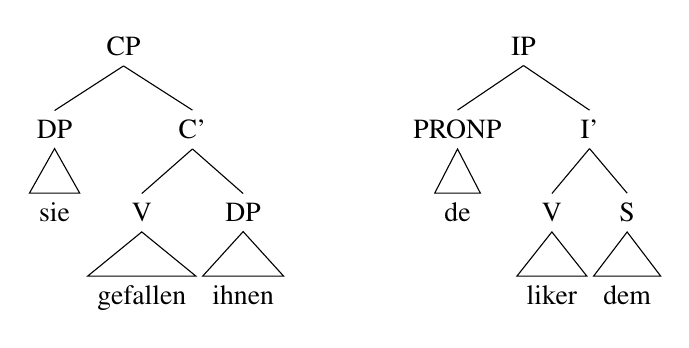
\begin{tikzpicture}
\Tree
[.CP
  [.DP \edge[roof]; {sie} ]   [.C'
    [.V
 \edge[roof]; {gefallen} ]     [.DP \edge[roof]; {ihnen} ]  
]]
\begin{scope}[shift={(2in,0in)}]
\Tree
[.IP
  [.PRONP \edge[roof]; {de} ] 
  [.I'
    [.V \edge[roof]; {liker} ] 
    [.S \edge[roof]; {dem} ] 
]]
  \end{scope}
\end{tikzpicture}

\avmoptions{}
\begin{avm}
\sort{$^{0}$}{\[ {\sc pred} `{\bf gefallen}<[1:{\it pro}],[2:{\it pro}]>'\\
{\sc topic} \sort{$^{1}$}{\[ {\sc pred} `{\it pro}'\\
{\sc ntype} \sort{$^{7}$}{\[ {\sc nsyn} pronoun\]}
\\
{\sc pron-type} pers, {\sc pron-form} sie, {\sc pers} 3,\\
{\sc num} pl, {\sc case} nom\]}
\\
{\sc tns-asp} \sort{$^{4}$}{\[ {\sc tense} pres, {\sc mood} indicative\]}
\\
{\sc obj-th} \sort{$^{2}$}{\[ {\sc pred} `{\it pro}'\\
{\sc ntype} \sort{$^{10}$}{\[ {\sc nsyn} pronoun\]}
\\
{\sc pron-type} pers, {\sc pron-form} sie, {\sc pers} 3,\\
{\sc num} pl, {\sc case} dat\]}
\\
{\sc subj} \[1\]\\
{\sc vtype} main, {\sc stmt-type} decl,\\
{\sc passive} -, {\sc clause-type} decl\]}
\end{avm}




\begin{avm}
\sort{$^{0}$}{\[ {\sc pred} `{\bf like}<[10:de],[11:de]>NULL'\\
{\sc tns-asp} \sort{$^{13}$}{\[ {\sc tense} pres, {\sc mood} indicative\]}
\\
{\sc topic} \sort{$^{10}$}{\[ {\sc pred} `{\bf de}'\\
{\sc ntype} \sort{$^{18}$}{\[ {\sc nsyn} pronoun\]}
\\
{\sc def} +, {\sc case} nom, {\sc ref} +,\\
{\sc pron-type} pers, {\sc pron-form} de, {\sc pers} 3,\\
{\sc num} pl\]}
\\
{\sc obj} \sort{$^{11}$}{\[ {\sc pred} `{\bf de}'\\
{\sc ntype} \sort{$^{45}$}{\[ {\sc nsyn} pronoun\]}
\\
{\sc ref} +, {\sc pron-type} pers, {\sc pron-form} de,\\
{\sc pers} 3, {\sc num} pl, {\sc def} +,\\
{\sc case} obl\]}
\\
{\sc subj} \[10\]\\
{\sc vtype} main, {\sc vform} fin, {\sc stmt-type} decl\]}
\end{avm}


\subsection{\textbf{SKRIV} døme med wager/3 og vedde/4 og gewettet/3 \textbf{:ROTETE:}}
\label{sec-3.15.5}


\subsection{\textbf{SKRIV} (reinskriv) \textbf{:ROTETE:}}
\label{sec-3.15.6}

Same globale tyding krev i det minste at, i situasjonen verbet
denoterer, speler deltakarane same rolle. Men dette er endå meir
abstrakt/semantisk enn (semantisk) argumentstruktur\ldots{}

Problem: ikkje-komposisjonell omsetjing. Same globale tyding. Det
treng ikkje vere berre pragmatisk forskjell--type \emph{kan du lukke døra}
vs \emph{lukk døra}, kor situasjon gjer setningane like--sidan me kan ha
konvensjonaliserte konstruksjoner på L1 kor heile tilsvarer enkeltord
på L2, a la japansk \emph{viss eg ikkje går på skulen så kan det ikkje vere} \~{}= \emph{eg må gå på skulen}. 

Ein føresetnad eg har, er at setningar som er samanstilte faktisk har
ein omsetjingsmessig korrespondanse (dette er min data). Så om eit par
av ytre predikat ikkje korresponderer er det au ein type data; nemleg
at me har ein omsetjingsmessig korrespondanse der det var ein mismatch
i ytre argumentstruktur. (Algoritmen bør då lagre slike mismatches
eksplisitt, ikkje berre la vere å lenkje, for det kan vere andre
grunnar til at det ikkje kom ei lenkjing. A la ekspertsystem: forklare
resonnementet.)

Alternativt ein konstruksjonslenkjing\ldots{} 

Kan au ha eit krav om at argstr til $PRED_{L1}$ er ein slags delmengd av
argstr til $PRED_{L2}$. 
\subsection{\textbf{SKRIV} True Arguments vs True Adjuncts, Pustejovsky \textbf{:ROTETE:}}
\label{sec-3.15.7}

\begin{itemize}
\item Treng døme først\ldots{}
\item Er «with Browne» eit Default Argument for «wager»?

\begin{itemize}
\item D-ARG: he built a house \underline{out of bricks}
\end{itemize}

\item Adjunkt plukker ut sine eigne roller, per definisjon, ved
     vedde/4 og wager/3 har me ein slik situasjon:
\begin{verbatim}
      vedde <—————wager >———<———wetten
             \____with_/     \__dass
\end{verbatim}

     Bottom-up-informasjon vil au vere naudsynt for dei 3 rollene
     som \emph{er} argument, sidan me kan ha vedde<1,2,3,4> og
     wager<a,b,c>with<d>, kor det er umogleg å seie om d skal på plass
     1,2,3 eller 4 (dvs. me kan ha vedde<a,b,c,d>, vedde<a,b,d,c>,
     vedde<a,d,b,c> og vedde<d,a,b,c> -- men sannsynlegvis er altså
     a,b,c i same rekkjefølgje uansett\ldots{})
\end{itemize}
\section{\textbf{SKRIV} Kan adjunkt lenkjast til nodar \underline{under} mor-lenkja?}
\label{sec-3.16}

Krav (vi) i \citet[s.~75]{dyvik2009lmp} krev at viss F$_s$ og F$_t$ er
lenkja, så kan ingen adjunkt D$_s$ til F$_s$ vere lenkja til nodar utanfor
F$_t$. Men kan ein D$_s$ lenkjast til ei dotternode av argument eller
adjunkt til F$_t$?

R$_t$ er dotter til F$_t$, og må då vere lenkja til ei dotter av F$_s$,
A$_s$. Då må au alle argument til R$_t$ vere lenkja til døtre av A$_s$, så
D$_s$ kan ikkje lenkjast til argument av dotternodar til F$_t$. Kva med
adjunkt? Om me finn eit ulenkja adjunkt til R$_t$ kan me heller ikkje
lenkje dette til D$_s$ ved krav (vi) igjen, sidan D$_s$ står utanfor
A$_s$.

Men om D$_t$ er ei ulenkja \emph{adjunkt}dotter av F$_t$, så vil døtre av
D$_t$ kunne lenkjast til D$_s$, så lenge D$_t$ forblir ulenkja. Me kan altså
sjå ned i adjunktdøtre av F$_t$ for å lenkje D$_s$. 

På same måte bør ein kunne rekursivt sjå ned i ulenkja adjunktdøtre av
R$_t$, men ein bør kanskje ikkje kunne lenkje så djupt uansett? Ikkje
automatisk, uansett.



Programmet mitt vil, gitt to initielle f-strukturar med
LPT-korrespondanse, finne alle moglege kombinasjonar av lenkjer som
inneheld alle argument og kanskje adjunkt, dvs. om me har

\begin{verbatim}
 F_s [ PRED p<1,2> ADJUNCT { 3 } ]
\end{verbatim}


\begin{verbatim}
 F_t [ PRED p<4> ADJUNCT { 5,6 } ]
\end{verbatim}


vil dette vere logisk moglege samanstillingar av «f-strukturdøtre»:

\begin{verbatim}
    (((1 . 4) (2 . 5)) ((1 . 4) (2 . 6)) ((1 . 5) (2 . 4))
     ((1 . 5) (2 . 6) (3 . 4)) ((1 . 6) (2 . 4)) ((1 . 6) (2 . 5) (3 . 4)))
\end{verbatim}


Me luker ut kombinasjonar som bryt med LPT-korrespondanse. Med full
informasjon bør me sjølvsagt berre ende opp med éin kombinasjon,
t.d. \texttt{((1 . 4) (2 . 5))}.

Så langt bør altså krav (i-iv) frå \citet{dyvik2009lmp} vere dekkja.

Me \underline{kan} krevje at f strukturane-til f strukturdøtre-kan lenkjast
rekursivt for at F$_s$ og F$_t$ skal lenkjast, t.d. både \texttt{(1 . 4)} og \texttt{(2 . 5)}. Men her kjem det (iallfall) to problem.


\subsection{1. Kausativar og inkorporering}
\label{sec-3.16.1}

Om me har 

\begin{verbatim}
 F_s [ PRED p<SUBJ, 1, 2> XCOMP 2[ PRED q<1> ] ]
\end{verbatim}


\begin{verbatim}
 F_t [ PRED pq<SUBJ,OBJ> ]
\end{verbatim}


kor pq er t.d. ein kausativ som tilsvarer \texttt{p<..., q>}, så vil me ikkje
kunne lenkje F$_s$ og F$_t$ sidan det bryt med krav (iii), F$_s$ har eit
argument for mykje. Men her vil det kanskje vere naturleg å ha ei
ein-mange-lenkje:

\begin{verbatim}
 ((F_s 2) . F_t)
\end{verbatim}


No kan me sjå på unionen av argument av F$_s$ (minus XCOMP) og argument
av XCOMP, alle argument i denne unionen må då ha LPT-korrespondanse
med argument/adjunkt av F$_t$, og alle argument av F$_t$ må ha
LPT-korrespondanse med argument/adjunkt av unionen.

Det same bør kanskje skje ved vanleg inkorporering av substantiv, då
må det altså vere mogleg å føye saman t.d. verb og objekt; ein
kombinasjon av dette og kausativ bør vel vere mogleg, t.d.

\begin{verbatim}
 F_s [ PRED la<SUBJ, 1>  XCOMP 2[ få<1, 3:pengar> ] ]
\end{verbatim}


\begin{verbatim}
 F_ t [ PRED belønn<SUBJ, 1> ]
\end{verbatim}


Igjen ser me på argument frå unionen av \texttt{(F\_s 2 3)} minus 2 og 3, og
om det er mogleg å lenkje dei til argument/adjunkt av F$_t$, og omvendt.

Men det bør kanskje vere grenser for kor langt samanføying kan gå… eg
kan ikkje tenkje meg at me vil lenkje \texttt{((F\_s 2) . F\_t)} eller \texttt{((F\_s 1 2) . F\_t)} her:

\begin{verbatim}
 F_s [ PRED p<…, 1> XCOMP 1[ PRED q<…, 2> XCOMP 2[ PRED r<…> ] ] ]
\end{verbatim}


\begin{verbatim}
 F_t [ PRED pr<…> ]
\end{verbatim}


\ldots{}men det kan jo hende det finst situasjonar der dette au vil vere
rett. Problemet er altså kor me skal setje grensene i
implementasjonen. Om me skal prøve å samanføye på alle moglege måtar
(altså, der me ikkje har informasjon om LPT), i tillegg til «vanlege»
lenkjer, blir det fort komputasjonelt vanskeleg. Me kan sjølvsagt snu
på LPT-kravet her, og seie at dette er berre lov der me har positiv
informasjon om LPT-korrespondanse, i staden for at det ikkje er lov om
me har motstridande LPT-informasjon, det vil nok hjelpe, men det er
vanskeleg å finne prinsipelle avgrensingar her. 
\subsubsection{\textbf{TOGROK} adjunkt bør ikkje samanføyast? eller?}
\label{sec-3.16.1.1}

Det einaste eg kan
tenkje meg er at adjunkt ikkje bør vere kandidatar for samanføying (i
såfall burde dei vel heller vore analysert som argument?).

\subsection{2. Adposisjonsobjekt}
\label{sec-3.16.2}


I følgjande setningspar har me eit objekt «sigarett» som svarer til
PP-en «sigaretze» («sigareti» + «ze»):

\begin{verbatim}
 Abrams veddet en sigarett med Browne på at det regnet.
 abramsi brouns daenajleva sigaretze, rom cvimda.
\end{verbatim}


\begin{verbatim}
 F_s [ PRED sigarett ]
\end{verbatim}


\begin{verbatim}
 F_t [ PRED ze<1> 1[ PRED sigareti ] ]
\end{verbatim}


F$_s$ og F$_t$ er døtre av dei ytre predikata i kvar setning, krav (iii)
seier at det må vere LPT-korrespondanse mellom desse for at me skal
kunne lenkje «veddet» og «daenajleva».  Her synest det feil å føye
saman «sigareti» og «ze», \texttt{(F\_s . (F\_t 1))}, sidan «sigarett» ikkje
inneheld informasjonen gitt av «ze».

Eg ser to løysingar. Me kan slakke på LMT-kravet ved å la \texttt{L'(F\_t) = \{sigaretze, ze\}} (evt. \texttt{\{sigaret, ze\}}), då kan me lenkje \texttt{(F\_s . F\_t)}, medan 1 er ulenkja.

Eller me kan lenkje \texttt{(F\_s . 1)}, kor me har skikkeleg
LMT-korrespondanse, men då må me slakke på (iii) og (iv), og altså ha
lov til å «hoppe over» ein f-struktur for å lenkje «veddet» og
«daenajleva». F$_t$ er då ulenkja.

For meg synest det mest naturleg å lenkje NP til PP, om ein skal
studere relasjonar mellom kasus, argumentstruktur og tematiske
roller. 
\subsubsection{\textbf{TOGROK} Eller finst det gode argument for å lenkje (F$_s$ . 1) ?}
\label{sec-3.16.2.1}


\section{\textbf{TOGROK} kva var poenget med dette? \textbf{:ROTETE:}}
\label{sec-3.17}

«etter og uten er dei einaste prep som tek setn utan å vere arg»
\section{\textbf{ULEST} Cyrus, FuSe-prosjektet \textbf{:ROTETE:}}
\label{sec-3.18}

\citet{cyrus2004apa}
«Abstract: We report on a recently initiated project which aims at
building a multi-layered parallel treebank of English and
German. Particular attention is devoted to a dedicated
predicate-argument layer which is used for aligning translationally
equivalent sentences of the two languages. We describe both our
conceptual decisions and aspects of their technical realisation. We
discuss some selected problems and conclude with a few remarks on how
this project relates to similar projects in the field.»
\section{\textbf{TODO} Konstruksjonar og komposisjonell inekvivalens}
\label{sec-3.19}

\xbar-teori føreset at det finst éi dotter i kvart ledd som kan
reknast som predikatet for dette leddet. Ei utfordring for
\xbar-baserte teoriar er då handsaming av \emph{komplekse predikat}. Desse
har fleire grammatiske element innanfor same ledd som alle bidrar med
«a non-trivial part of the information of the complex predicate»
\citep{alsina1997cp}. I LFG er det ein føresetnad at me berre har éin
\textsc{pred} ytterst i kvar f-struktur; ulike mekanismar har blitt
føreslått for å handsame dette fenomenet.

I omsette tekster kan me få eit analogt problem:

\ex. It can't be done \\
     Det lar seg ikke gjøre

Her vil ytre predikat i f-strukturen på norsk vere
`la<det$_1$,XCOMP>PRO', kor XCOMP[PRED `gjøre<NULL,det$_1$>NULL'].

På engelsk får me `can<XCOMP,it$_2$>', kor
XCOMP[PRED `do<NULL,it$_2$>']. 


Skal me lenkje orda \emph{can} og \emph{la}? På \emph{heile konstruksjonen} finn me
iallfall eit omsetjingsforhold:


\begin{center}
\begin{tabular}{lll}
 It can't be done                    &  Det lar seg ikke gjøre               &      \\
 can't be done                       &  lar seg ikke gjøre                   &      \\
 be done                             &  gjøre                                &  s?  \\
 \_{} can't be VPASS                 &  \_{} lar seg ikke VPASS              &  ??  \\
 \_$_{1}$ can \_$_{2}$ be VPASS$_3$  &  \_$_{1}$ lar seg \_$_{2}$ VPASS$_3$  &  ??  \\
\end{tabular}
\end{center}




(kan me få den siste generaliseringa frå trebanken?)


\section{\textbf{SKRIV} definer sitering frå MRS-suiten \textbf{:ROTETE:}}
\label{sec-3.20}

\section{\textbf{SKRIV} setning 7 i MRS-suiten \textbf{:ROTETE:}}
\label{sec-3.21}



  

Ein samanstilling bør i det minste gi følgjande:


\begin{center}
\begin{tabular}{ll}
 abramsi brouns daenajleva sigaretze, rom cvimda  &  Abrams veddet en sigarett med Brown på at det regnet  \\
 abramsi brouns daenajleva sigaretze              &  Abrams veddet en sigarett med Brown                   \\
 brouns daenajleva sigaretze                      &  veddet en sigarett med Brown                          \\
 daenajleva sigaretze                             &  veddet (en) sigarett (på)                             \\
 daenajleva                                       &  veddet                                                \\
 sigaretze                                        &  (en) sigarett (på)                                    \\
 rom cvimda                                       &  at det regnet                                         \\
 cvimda                                           &  (det) regnet                                          \\
 abramsi                                          &  Abrams                                                \\
 brouns                                           &  Brown                                                 \\
\end{tabular}
\end{center}


 
\section{\textbf{TOGROK} og så finst jo større forskjellar, stilistiske osb\ldots{} \textbf{:ROTETE:}}
\label{sec-3.22}


\section{\textbf{TOGROK} prosessering, kognitive modellar? \textbf{:ROTETE:}}
\label{sec-3.23}

finne empiri frå korleis menneske samanstillar? (dvs., korleis skjer
omsetjing)

\begin{itemize}
\item \citet{maier2009sis}, \href{http://linguistlist.org/issues/20/20-1786.html}{http://linguistlist.org/issues/20/20-1786.html}
\end{itemize}
«cross-linguistic structural phenomena in the language production of
bilinguals in the specific context of translation.»

\begin{itemize}
\item \href{http://www.linguistlist.org/pubs/diss/browse-diss-action.cfm?DissID=143}{http://www.linguistlist.org/pubs/diss/browse-diss-action.cfm?DissID=143}
\item \href{http://books.google.com/books%3Fhl%3Dno&lr%3D&ie%3DUTF-8&id%3DhHFoJguRE4oC&oi%3Dfnd&pg%3DPA141&dq%3Dprocessing%2Btranslation%2Bpsycholinguistic%2Bsyntax&ots%3DNUlz1ebVnE&sig%3DrkMwuX59RoIikvTYGq23HNkYtzc}{books.google bialystok????lpb}: «Translation has been called
  ``interlanguage paraphrase''», «a metalinguistic skill». «Paraphrasing
  consists in finding the meaning of two compared sequences and
  showing its equivalence, and this identification constitutes a
  judgment on the sequences»[s.\~{}151]
\item \href{http://books.google.com/books%3Fhl%3Dno&lr%3D&ie%3DUTF-8&id%3DCZXcTzFLDuwC&oi%3Dfnd&pg%3DPA17&dq%3Dprocessing%2Btranslation%2Bpsycholinguistic%2Bsyntax&ots%3DFUm_X5VCeu&sig%3DNoHLNrNxq7bGNAcsRda8RWNDyOY}{books.google house????iic}: «The process of translation, particularly
  if successful, necessitates a complex text and discourse
  processing. The process of interpretation performed by the
  translator on the source text might lead to a TL text which is more
  redundant than the SL text. This argument may be stated as ``the
  explicitation hypothesis'', [\ldots{}] especially marked in the work of
  ``non professional'' translators» [s.\~{}19--20]
\item Hutchinson: «What is a grammatical sentence?» (vanskeleg å unngå
  \emph{talaren} i akseptabilitetvurderingar); kva \underline{er} ei frasesamanstilling,
  sånn ute i naturen?
\end{itemize}
\section{\textbf{TOGROK} Retningslinjer for samanstilling \textbf{:ROTETE:}}
\label{sec-3.24}

Ved korpusbygging er det vanleg at retningslinjer for samanstilling
blir utvikla \emph{etter kvart som ein finn problem}\ldots{} (det er vanskeleg å
seie noko \emph{a priori} om kva for vanskar ein kan finne).



\chapter{Korleis fungerer implementasjonen min}
\label{sec-4}

For å finne ut av kor godt krava i forrige kapittel fungerer til å
avgrense kva for lenkjer som er moglege, har eg implementert dei etter
beste evne i eit Lisp\footnote{Common Lisp er m.a. nytta i LFG Parsebanker
        \citep{rosen2009lpt}. }-program.

\fxnote{intro todo} Ei implementering gjer det svært synleg om det
finst manglar i eit formelt krav, eller om noko ikkje er godt nok
spesifisert.

Programmet \texttt{lfgalign}\footnote{Tilgjengeleg frå \href{http://github.com/unhammer/lfgalign}{http://github.com/unhammer/lfgalign} som fri og
       open programvare under GNU General Public License. } tek inn LFG-analysane av to
setningar som me av uavhengige grunnar trur er omsetjingar av
kvarandre. LFG-analysane må vere disambiguerte og i Prolog-formatet
frå XLE\footnote{Dokumentert på
       \href{http://www2.parc.com/isl/groups/nltt/xle/doc/xle.html}{http://www2.parc.com/isl/groups/nltt/xle/doc/xle.html}. Importeringa
       til Lisp-strukturar handterer «pakka representasjonar» og
       kjenner igjen ekvivalensforhold (t.d. der fleire variablar
       refererer til same f-struktur, eller til same analyseval); men
       filene eg har testa utnyttar ikkje det fulle spennet til
       formatet, så det finst ganske sikkert feil. }. Programmet les inn dei to filene og opprettar ein
intern representasjon av LFG-analysen.

Me kan i tillegg gi programmet informasjon om kva for ord-omsetjingar
me ser på som lingvistisk prediktable (t.d. informert av
omsetjingstabellen frå eit automatisk ordsamanstillingsprogram, eller
av handskrivne omsetjingsordbøker).

\section{f-struktursamanstilling}
\label{sec-4.1}

\fixme{intro, c-str er derivativ}

Hovudalgoritmen er vist i kodefigur \ref{algo:f-align}. Funksjonen
\texttt{f-align} returnerer ei mengd med moglege samanstillingar. Kvar
samanstilling er ei mengd med par av f-strukturar. Eit par $(F_s,F_t)$
representerer ei lenkje frå ein f-struktur på kjeldespråket, til ein
f-struktur på målspråket. Me føreset at dette paret har
LPT-korrespondanse\footnote{Når eg her skriv at to f-strukturar har LPT-korrespondanse,
        meiner eg sjølvsagt at ordformen til PRED-verdien til kvar
        f-struktur har LPT-korrespondanse. }, dette blir sjekka før alle kall på
\texttt{f-align}.

Hjelpefunksjonen \texttt{argalign} (som igjen kallar \texttt{argalign-p}, vist i
kodefigur \ref{algo:argalign-p}) gir alle moglege
«argumentpermutasjonar», dvs. moglege kombinasjonar av lenkjer mellom
argumenta til $F_s$ og $F_t$ som tilfredsstiller kravet om
LPT-korrespondanse, men utan å sjekke at desse argumenta igjen kan
samanstillast. Funksjonen prøver å lenkje kvart argument til eit
argument eller eit adjunkt, men gir ingen lenkjer mellom to
adjunkt. Funksjonen gir heller ikkje kombinasjonar der minst eitt
argument ikkje er lenkja -- alle kombinasjonane må inkludere alle
argument frå $F_s$ og $F_t$, jf. krav (iii) og (iv) i
\citet[s.~75]{dyvik2009lmp}; krav (i) er tautologisk oppfylt, medan me
som nemnt føreset at krav (ii) er oppfylt før alle kall på \texttt{f-align}.

Eit døme: viss $F_s$ har argumenta \SUBJ og \OBJ og ingen adjunkt, og
$F_t$ har argumentet \SUBJ og eitt adjunkt \ADJ, der alle
ord-omsetjingar er moglege, vil \texttt{argalign} gi dei to samanstillingane
$\{(\SUBJ,\SUBJ), (\OBJ,\ADJ)\}$ og $\{(\SUBJ,\ADJ),
(\OBJ,\SUBJ)\}$. Viss adjunktet til $F_t$ ikkje fantest, eller ikkje
hadde LPT-korrespondanse med nokon av argumenta til $F_s$, får me
ingen samanstillingar; medan viss berre $(\SUBJ,\SUBJ)$ ikkje hadde
LPT-korrespondanse, får me berre ut den siste samanstillinga.

Funksjonen \texttt{f-align} går så gjennom kvar lenkje i kvar
argumentpermutasjon, og prøver å kalle \texttt{f-align} på alle
lenkjene. Sidan lenkjene som \texttt{argalign} gir har LPT-korrespondanse,
vil alle f-strukturane i dei rekursive kalla i \texttt{f-align} ha
LPT-korrespondanse. Eit rekursivt kall kan gi nye samanstillingar i
dei indre f-strukturane, viss dei relevante krava er oppfylte. Då
lagrar me samanstillinga av understrukturane saman med paret
$(F_s,F_t)$.

Det er mogleg at ei lenkje frå éi samanstilling kan finnast i andre
samanstillingar, difor lagrar me alle delvise samanstillingar i
tabellen $aligntable$. Dette føreset sjølvsagt at
\texttt{f-align}$(s,t)$ er uavhengig av konteksten rundt, t.d. at
mengda av samanstillingar som kjem ved å lenkje subjektet til $F_s$
mot subjektet til $F_t$ er uavhengig av om objektet til
$F_s$ er lenkja mot eit objekt eller eit adjunkt osb. av
$F_t$. \fxnote{nemne dette «kravet» / føresetnaden i kapittelet
over}  

     \begin{algorithm}[]
      \caption{f-align($F_s$, $F_t$)}
      \label{algo:f-align}
      
      $alignments \gets \emptyset$  \;
      \ForAll{argperm in argalign($F_s$, $F_t$)} {
        $p \gets \emptyset$ \;
         \ForAll{$A_s$, $A_t$ in argperm} {
           \uIf{unset(aligntable[$F_s$,$F_t$])} {
           aligntable[$F_s$,$F_t$] $\gets$ f-align($A_s$, $A_t$)\;
           }
          add aligntable[$F_s$,$F_t$] to $p$\;
        }
        add $p$ to $alignments$ \;
       }
       \Return $((F_s, F_t), alignments)$ \;
       \end{algorithm}
    
    
    
      \begin{algorithm}[]
      \caption{argalign-p($args_s$, $adjs_s$, $args_t$, $adjs_t$)}
      \label{algo:argalign-p}
    
      \SetKwComment{Comment}{ // }{}
      \SetKwInOut{Input}{usage}
      \Input{Kalt av argalign slik: \\ argalign-p(arguments($F_s$),
      adjuncts($F_s$), arguments($F_t$), adjuncts($F_t$))}
      \BlankLine
    
    
     $a \gets \emptyset$\;
     \uIf{$args_s$} {
           $s \in args_s$\;
           \ForAll{$t \in args_t$ \textbf{where} LPT($s$,$t$)} {
               \lForAll{$p \in$ argalign-p($args_s-\{s\}$, $adjs_s$, $args_t-\{t\}$,$adjs_t$)}{
  add $\{(s,t)\} \bigcup p$ to $a$\;
             }
            }
           \ForAll{$t \in adjs_t$ \textbf{where} LPT($s$,$t$)} {
               \lForAll{$p \in$ argalign-p($args_s-\{s\}$, $adjs_s$, $args_t$,$adjs_t-\{t\}$)}{
  add $\{(s,t)\} \bigcup p$ to $a$\;
                }
           }
             \Return $a$\;
         }
          \uElseIf{$args_t$} {
            \uIf{$adjs_s$}{
                $s \in adjs_s$\;
           \ForAll{$t \in args_t$ \textbf{where} LPT($s$,$t$)} {
               \lForAll{$p \in$ argalign-p($args_s$, $adjs_s-\{s\}$, $args_t-\{t\}$,$adjs_t$)}{
  add $\{(s,t)\} \bigcup p$ to $a$\;
             }
            }
             \Return $a$\;
        }\uElse{
              \Return $\emptyset$  \Comment*[l]{Fail}
            }
          }
        \uElse {
          \Return \{$\emptyset$\} \Comment*[l]{End}
        }     
      \end{algorithm}

Sjølv om det er krav om LPT-korrespondanse mellom kvart argument og
eit argument/adjunkt, er det ikkje eit krav om at alle desse para
tilfredsstiller alle lenkjingskrava for at $F_s$ og $F_t$ skal
lenkjast. Viss \texttt{f-align}$(\OBJ,\ADJ)$ frå dømet over gir null,
og ikkje kan lenkjast, medan \texttt{f-align}$(\SUBJ,\SUBJ)$ kan
lenkjast, får me ei delvis lenkjing av argumenta i den 

  Krav (iii) og (iv) i
\citet[s.~75]{dyvik2009lmp} seier at det må vere LPT-korrespondanse
mellom

Om me i tillegg krev at f-strukturane deira kan samanstillast kan me
utelukke lenkjing av $F_s$ og $F_t$ nedanfor:

\begin{verbatim}
 F_s[ PRED planlegge<eg,1>      F_t[ PRED plan<I,3>
      XCOMP 1[gi (opp)]      ]       XCOMP 3[ give<I,him,it> ]
\end{verbatim}


\fixme{Skal eg krevje dette? Foreløpig har eg }

\section{Kan me gjere f-struktursamanstillinga fullstendig bottom-up?}
\label{sec-4.2}

Ein alternativ metode er å byrje med alle moglege permutasjonar av
LPT-korrespondansar, og så sile ut dei som ikkje svarer til krava. Men
dette er problematisk, sidan avskjeringa då skjer så seint at
utrekningane for lengre setningar blir ganske umogleg.

Me må i alle tilfelle vere klar for ei setning der alle ord er ukjende
(me har ingen informasjon om LPT-korrespondanse), slik at kvart
kjeldeord kan lenkjast til kvart målord. Viss båe setningane er 4 ord,
får me 16 moglege samanstillingar der alle ord er med i nøyaktig éi
lenkje ($2^l$, kor $l$ er setningslengd). Men ofte har me
null-lenkjer, me må altså i tillegg tillate samanstillingar der minst
eitt ord er ulenkja, utan at me treng å vite kva for ord det er; med
desse kortare listene inkludert får me endå fleire moglege
samanstillingar per setning (4 ord gir 26, 8 ord gir 2186 moglege
samanstillingar). Sjølv om me heile tida vel dei samanstillingane som
lenkjar flest ord, ville maskinen raskt fått problem. I tillegg har me
problemet med 1-mange-lenkjer, som skaper endå fleire moglege
samanstillingar.
\subsection{notat \textbf{:ROTETE:}}
\label{sec-4.2.1}

Intuition: Starting the alignment from outers and then going
inwards should have the effect that  

\begin{enumerate}
\item we don't get `crossing' alignments, as we would have if 
   a-d and b-c where tab$_s$:[a [b ]] tab$_t$:[c [d ]], and
\item we prioritise alignments of outer elements with outer 
   elements.
\end{enumerate}
However, it might turn out to be really hard in practice to keep
possible pairings prioritised when aligning. Eg. if we have

tab$_s$:[a [b]] tab$_t$:[c [d [e]] [f [g]]
and all LPT's are allowed except a-d, do we go
a-c,a-e,a-f,a-g
or
a-c,a-f,a-e,a-g 
or 
a-c,a-f,a-g,a-e (here counting e as deeper than g)
?

And if tab$_s$ were [a [b]] [h [i]], when do we start considering h?

----

The alternative to ordering is of course just trying all permutations
of LPT-pairings. But would it still be simplest to follow some sort of
ordering? And how do we prioritise the full over the half-finished
alignments?

Proposal: do all pairings. Start with a pair of unreferenced-preds,
aligning inwards.

Another difficulty is that we can merge certain pairings, eg. where we
have a single causative PRED that aligns to a make PRED and a do PRED,
or an object PRED that's incorporated into an `action'
PRED (`bilvaskingen'). 

Proposal: `LPT-permute' churns out all configurations of single
pairings allowed by LPT, while a `merge' function creates new possible
configurations (pushed last in the queue) based on sane merges. So
far, I don't think we'll want to merge where where two PRED's are on
the same level (eg. a subject and an object of the same PRED we
wouldn't merge), but a PRED and XCOMP (causative) or a PRED and its
object (`bilvaskingen') would be mergeable, these have exactly one
level between them (ie. one is the parent of another). I'm not sure
that we want to stop there though (we might want to go both deeper in
the f-structure and wider, ie. merge a pred with both its subject and
its object, or with both its daughter and granddaughter); but we can
leave that for later probably. ADJUNCTs should probably be mergeable
too.



\section{merge}
\label{sec-4.3}

filene 
\begin{verbatim}
 ((tab_s (open-and-import "dev/TEST_argadj_s.pl"))
  (tab_t (open-and-import "dev/TEST_argadj_t.pl")))
\end{verbatim}

viser at me kan trenge samanføying av pred på ulike nivå.

``sigaretten'' og ``sigaretze'' er ikkje på same nivå i dei respektive
f-strukturane, me har
\begin{verbatim}
 0[ PRED vedde<28,29,27,30>
    29[ PRED sigarett<> ] ]
\end{verbatim}

og
\begin{verbatim}
 0[ PRED da-najleveba<37,10,46>
    ADJUNCT { 2 }
    2[ ze<5>
       OBJ 5[ sigareti ] ] ]
\end{verbatim}


\section{gjer ikkje dette lenger \textbf{:ROTETE:}}
\label{sec-4.4}

\texttt{lfgalign} kan i tillegg ta inn ein representasjon av moglege
LPT-korrespondansar.

LPT-korrespondansane utgjer utgangspunktet for samanstillinga. 

Der det ikkje finst informasjon om eit ord i LPT-basen, føreset me at
alle ord kan lenkjast til dette. Pronomen/pro-element og
substantiv/pronomen kan alltid lenkjast.

\texttt{permute} finn alle moglege permutasjonar av 1-1
LPT-korrespondansar. 

Dette blir sendt gjennom \texttt{merge} som finn moglege
mange-til-mange-korrespondansar av PRED-element. Moglege samanføyingar
er: PRED til (X)COMP-dotter, ADJUNCT, \ldots{}.

Så blir den utvida mengda med PRED-korrespondansar sendt vidare til
eit filter som sjekker om skrankane er oppfylte.

\chapter{Resultat av å automatisk samanstille norske og georgiske setningar}
\label{sec-5}

\begin{itemize}
\item om kjeldematerialet
\item manglar med implementasjonen
\item samanlikning av lenkjing basert på f-struktur og lenkjing basert
     på N-gram
\end{itemize}
\section{\textbf{TOGROK} korleis gjenfinne there is/es gibt? \textbf{:ROTETE:}}
\label{sec-5.1}

\begin{enumerate}
\item N-gram kjem like ofte som heile konstruksjonen, då kan dette
   gjenfinnast

\begin{itemize}
\item dvs., \emph{there is NP/es gibt NP}-samanstilling kjem like ofte som
     \emph{there is} eller \emph{es gibt} førekjem. Eit TigerXML-type søk etter
     \emph{there is NP/es gibt NP} burde jo vere mogleg, sjekk om dette er
     delmengd av \emph{there is/es gibt}. * Avslutning
\end{itemize}

\end{enumerate}
\bibliographystyle{apacite}
\bibliography{master}
























\end{document}